%!TEX TS-program = xelatex
%!TEX encoding = UTF-8 Unicode

\documentclass[tikz,border=1]{standalone}
\usepackage{pgfplots}

\begin{document}
  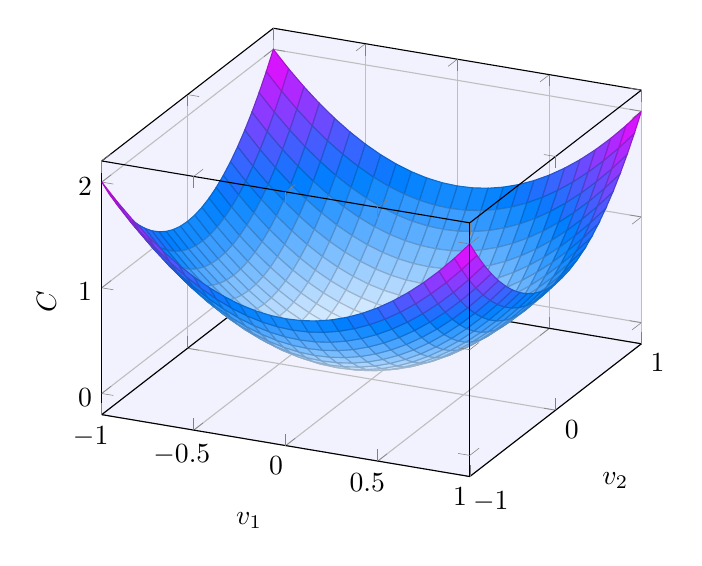
\begin{tikzpicture}
    % FIXME: rotate the zlabel, change plot color, and move z axis to right
    \begin{axis}[
      %title={$x^2 + y^2$},
      3d box=complete,
      grid=major,
      axis background/.style={fill=blue!5},
      xlabel=$v_1$,
      ylabel=$v_2$,
      zlabel=$C$,
      colormap/cool]
      \addplot3[surf,domain=-1:1] {
        x*x + y*y
      };
    \end{axis}
  \end{tikzpicture} 
\end{document}
